\documentclass[t]{beamer}


%useful packages
\usepackage{color,soul}
\usepackage{amsmath,amsthm,amscd,amssymb,bm}
\usepackage{hyperref}
\usepackage[utf8]{inputenc}
\usepackage{enumerate}
\usepackage{xcolor}


\let\OLDitemize\itemize
\renewcommand\itemize{\OLDitemize\addtolength{\itemsep}{10pt}}


%personal definitions and commands
\newcommand{\R}{\mathbb{R}} 
\newcommand{\E}{\mathbb{E}}
\newcommand{\V}{\mathbb{V}}
\newcommand{\C}{\mathbb{C}}
\newcommand{\Prob}{\mathbb{P}}
\newcommand{\e}{\epsilon}
\newcommand\numberthis{\addtocounter{equation}{1}\tag{\theequation}} %allows numbering of single equations in align* environment
\newcommand{\mtx}[1]{\ensuremath{\bm{\mathit{#1}}}}
\newcommand{\B}{\hat{\boldsymbol{\beta}}}
\newcommand{\Cov}{\mathbb{C}\text{ov}}
\newcommand{\N}{\mathcal{N}}


% \usepackage{beamerthemesplit} // Activate for custom appearance

\title{Chatterjee (2018), `Market Power and Spatial Competition in Rural India'}
\author{Nishaad Rao and Anirudh Yadav}
\date{\today}

\begin{document}

\frame{\titlepage}

\iffalse
\frame{\frametitle{Outline}
  \begin{enumerate}    
  \item Motivation and overview
  \item Reduced-form evidence
  \item Model
  \item Counterfactuals 
  \end{enumerate}
}


\frame{\frametitle{Motivation}
\begin{itemize}
\item Indian farmers are very poor (medium annual income $\approx \$365$).
\pause
\item Low farmer revenue partly due to the low prices they receive
\pause
\item Intermediaries (main buyers of crops) have monopsony power due to government regulations
\pause
\item Farmers are mandated to sell crops to licensed intermediaries at government-designated marketplaces \textit{in their own state}.
\end{itemize}
}

\frame{\frametitle{Questions}
\begin{enumerate}
\item Does more spatial competition between intermediaries raise farmer prices? \uncover<2->{\textbf{Yes.}}
\item How does removing the interstate trade restriction affect farmer prices/incomes/production? \\
\uncover<3->{\textbf{prices} $\uparrow$ \textbf{11\%}, \textbf{output} $\uparrow$ \textbf{7\%} }
\end{enumerate}
}

\frame{\frametitle{Institutional setting}
\begin{itemize}
\item State-level legislation (APMC Acts) mandate that the first sale of crops after harvest must be at government-designated marketplaces, and buyers must obtain a license.
\pause
\item Effectively prohibits farmers from selling crops in neighbouring states.
\pause
\item Reduces competition between marketplaces across state borders.
\pause
\item Treat each physical marketplace as having only one intermediary buyer.
\end{itemize}

}

\frame{\frametitle{Empirical methodology}
\begin{itemize}
\item Measure of spatial competition faced by a market $m$:
\begin{align*}
\text{comp}_m = \sum_{j \in \mathcal{M}/\{m\}} \left\{ \frac{1}{\text{distance}_{mj}}\right\}\bm{1}[\text{$m$ and $j$ are in the same state}]
\end{align*}
\pause
\item Analogous measure of interstate spatial competition:
\begin{align*}
\text{comp}'_m = \sum_{j \in \mathcal{M}/\{m\}} \left\{ \frac{1}{\text{distance}_{mj}}\right\}\bm{1}[\text{$m$ and $j$ not in the same state}]
\end{align*}
\end{itemize}

}

\frame{\frametitle{Example}
\begin{figure}
\centering
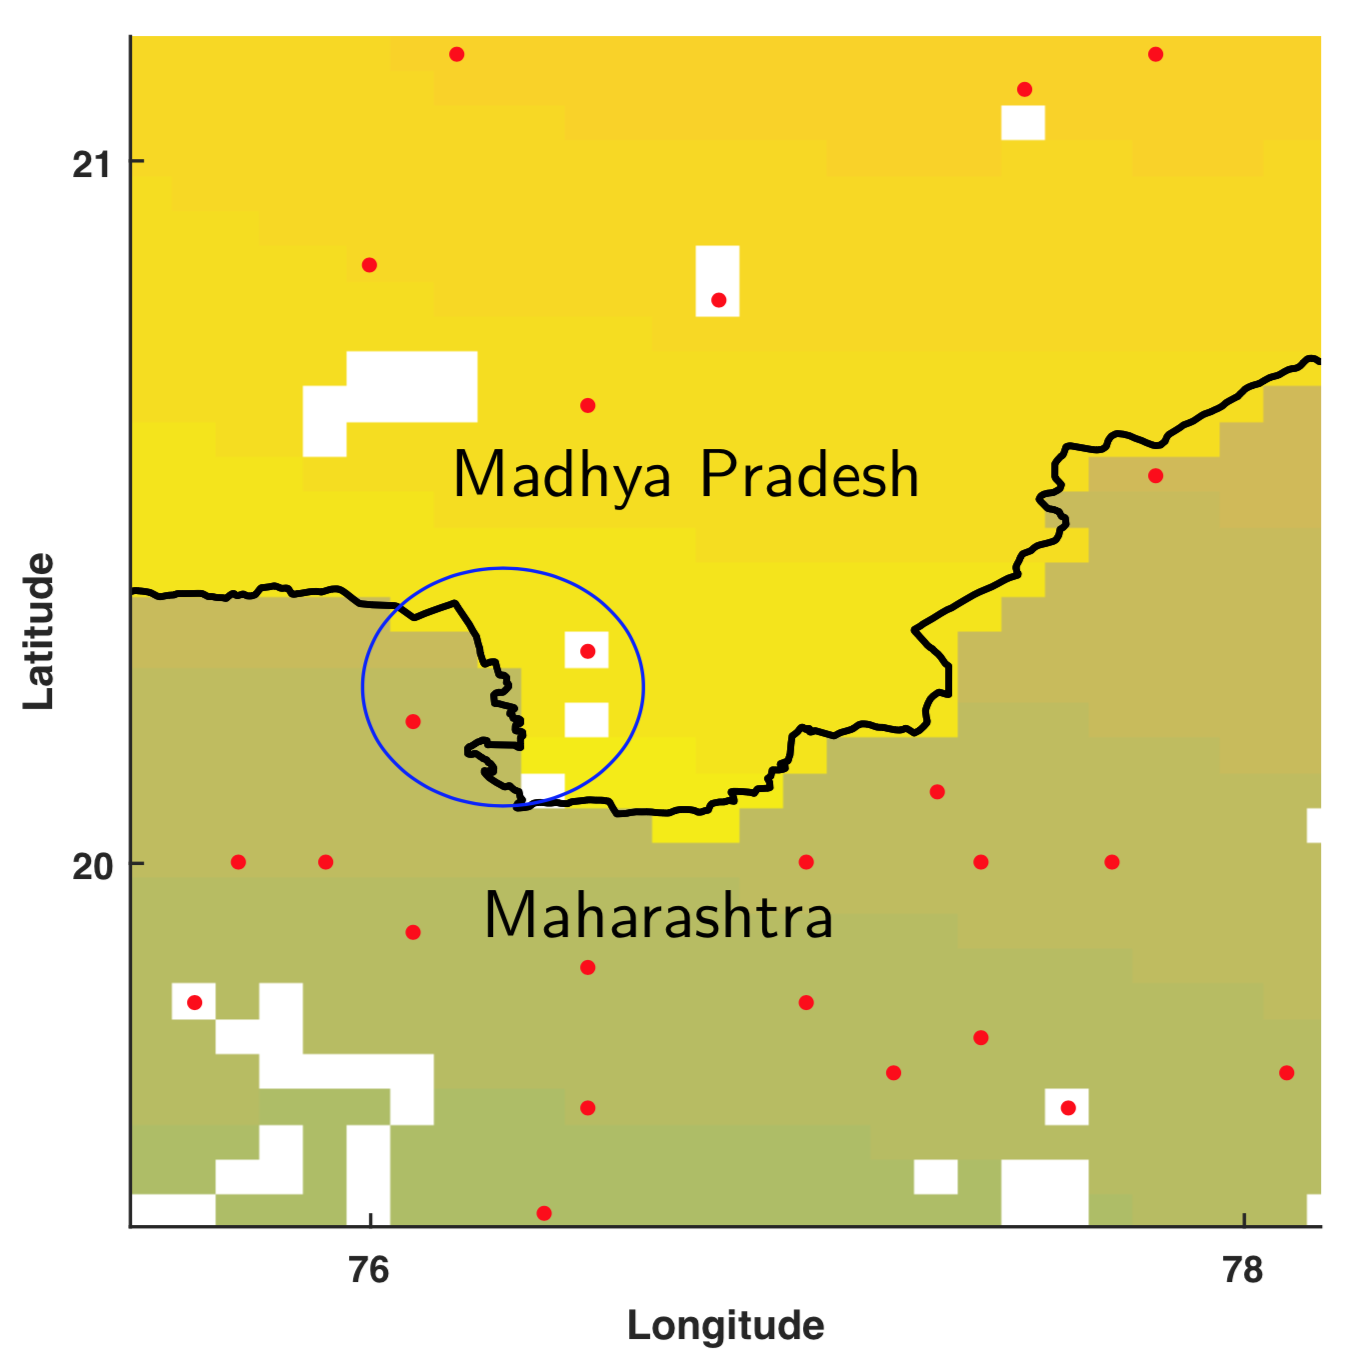
\includegraphics[width=0.7\textwidth]{example}
\end{figure}
}

\frame{\frametitle{Empirical methodology}
\begin{itemize}
\item Main specification:
\begin{align*}
\log p^f_{cmdst} =& \beta_0 + \beta_1 \text{comp}_m + \beta_2 \text{comp}'_m + \mtx{X}'_{cdt}\beta_3 \\
&+ \gamma_t + \gamma_c + \gamma_s + \e_{cmdt}
\end{align*}
where $p^f_{cmdst}$ is the price a farmer receives for crop $c$, at market $m$, in district $d$, state $s$, and month $t$.
\pause
\item Sample: 10 years (2005--2014), 2978 markets.
\end{itemize}

}

\frame{\frametitle{Empirical results}
\centering
\begin{table}
\begin{tabular}{lrr}
 & $\hat{\beta}_1$ & $\hat{\beta}_2$\\
 \hline
Point estimate &0.0163 & $-0.0005$\\
Std. err. & 0.0043 & 0.0012
\end{tabular}
\end{table}
\pause
\begin{itemize}
\item Greater spatial competition increases farmer prices!
\end{itemize}

}
\fi

\frame{\frametitle{Environment}
\begin{itemize}\setlength{\itemsep}{10pt}
\item $S$ regions (independent for now)
\item One crop (we'll add more later)
\item Within each region,
\begin{itemize}\setlength{\itemsep}{5pt}
\item farmers, $f\in \{1,...,F\} \equiv \mathcal{F}$
\item intermediares, $m \in  \{1,...,M\} \equiv \mathcal{M}$
\end{itemize}
\item Iceberg trade costs: $\tau_{fm}>1$.
\item Partial equilibrium (demand side is exogenously given)
\end{itemize}

}

\frame{\frametitle{Technology}
\begin{itemize}\setlength{\itemsep}{10pt}
\item Farmers have Cobb-Douglas production technology,
\begin{align*}
y_f = \tilde{A}_f\left(h_f^\gamma l_f^\nu \prod_{k=1}^K(x_f^k)^{\alpha_k}\right)
\end{align*}
\begin{itemize}\setlength{\itemsep}{10pt}
\item $\{x^k\}$ intermediate inputs, prices $\{w^k\}$ (exogenously given)
\item $h_f$ and $l_f$ are endowments of land and labor (i.e. fixed).
\end{itemize}

\end{itemize}

}

\frame{\frametitle{Market choice}
\begin{itemize}\setlength{\itemsep}{10pt}
\item Farmer's problem is to choose the market $m$ that maximizes profit (note the trade cost):
\begin{align*}
\max_{m \in \mathcal{M}} \left\{\frac{p^f(m)y_f}{\tau_{fm}}\right\}
\end{align*}
\end{itemize}
}

\frame{\frametitle{Price determination}
\begin{itemize}\setlength{\itemsep}{10pt}
\item Once farmer $f$ reaches market $m$, all costs are sunk.
\item Farmer's price is determined via Nash Bargaining.
\item Farmer's outside option:
\begin{align*}
\underline{p}(m) = \max_{k \in \mathcal{M} \backslash \{m\}} \left\{\frac{p^f(k)}{\tau_{mk}}\right\}
\end{align*}
\item Intermediary's outside option is zero.
\end{itemize}
}

\frame{\frametitle{Price determination: Nash bargaining}
\begin{itemize}\setlength{\itemsep}{10pt}
\item NB outcome is the solution to
\begin{align*}
\max_{\lambda}\text{ }  (\lambda - \underline{p}(m)q_m)^\delta(p^r_mq_m - \lambda)^{1-\delta}
\end{align*}
\begin{itemize}\setlength{\itemsep}{10pt}
\item $\lambda$ is farmer's income
\item $p^r_m$ is the retail price (exogenous)
\end{itemize}
\end{itemize}
}


\frame{\frametitle{Equilibrium}
Set of farmer prices $p^f(\cdot)$, intermediate input choices $\{x^k_f\}_{k\in \mathcal{K}, f\in \mathcal{F}}$, and the optimal market choice of each farmer $\{\mu(f)\}_{f \in \mathcal{F}}$:
\begin{enumerate}\setlength{\itemsep}{10pt}
\item Farmers maximize profits;
\item Farmers optimally choose the market to sell their output;
\item At each market, the farmer's price is determined by the NB solution, assuming that NB in all other markets have reached an agreement.
\end{enumerate}

}

\frame{\frametitle{Equilibrium -- solution}
\begin{itemize}\setlength{\itemsep}{10pt}
\item Solution to NB problem:
\begin{align*}
p^f(m) = (1-\delta) \underline{p}(m) + \delta p^r_m
\end{align*}
using $p^f(m)  = \lambda / q_m$.
\item System of $M$ equations in $M$ endogenous variables $\{p^f(m)\}_{m \in \mathcal{M}}$
\item \textbf{T1}: Equilibrium exists and is unique.
\item \textbf{L1}: Given retail prices, removing the interregional trading restriction improves farmer prices.\\
$\implies$ Intuition: farmer's outside option is better!
\end{itemize}
}

\frame{\frametitle{Taking model to the data}
\begin{itemize}\setlength{\itemsep}{10pt}
\item Expand to include multiple crops and time periods; system of $M \times C \times T$ equations/variables.
\item Semi-annual data (7 years): market locations, farmer prices and retail prices for each crop, district-level crop choice.
\item Estimation: (i) parameterize $\tau$; (ii) estimate $\delta$ + trade cost parameters using SMM.
\item Calibrate other parameters $(\gamma, \nu)$.
\end{itemize}

}

\frame{\frametitle{Counterfactual \#1: changing farmers' outside option}
\pause
\begin{figure}[htbp]
\centering
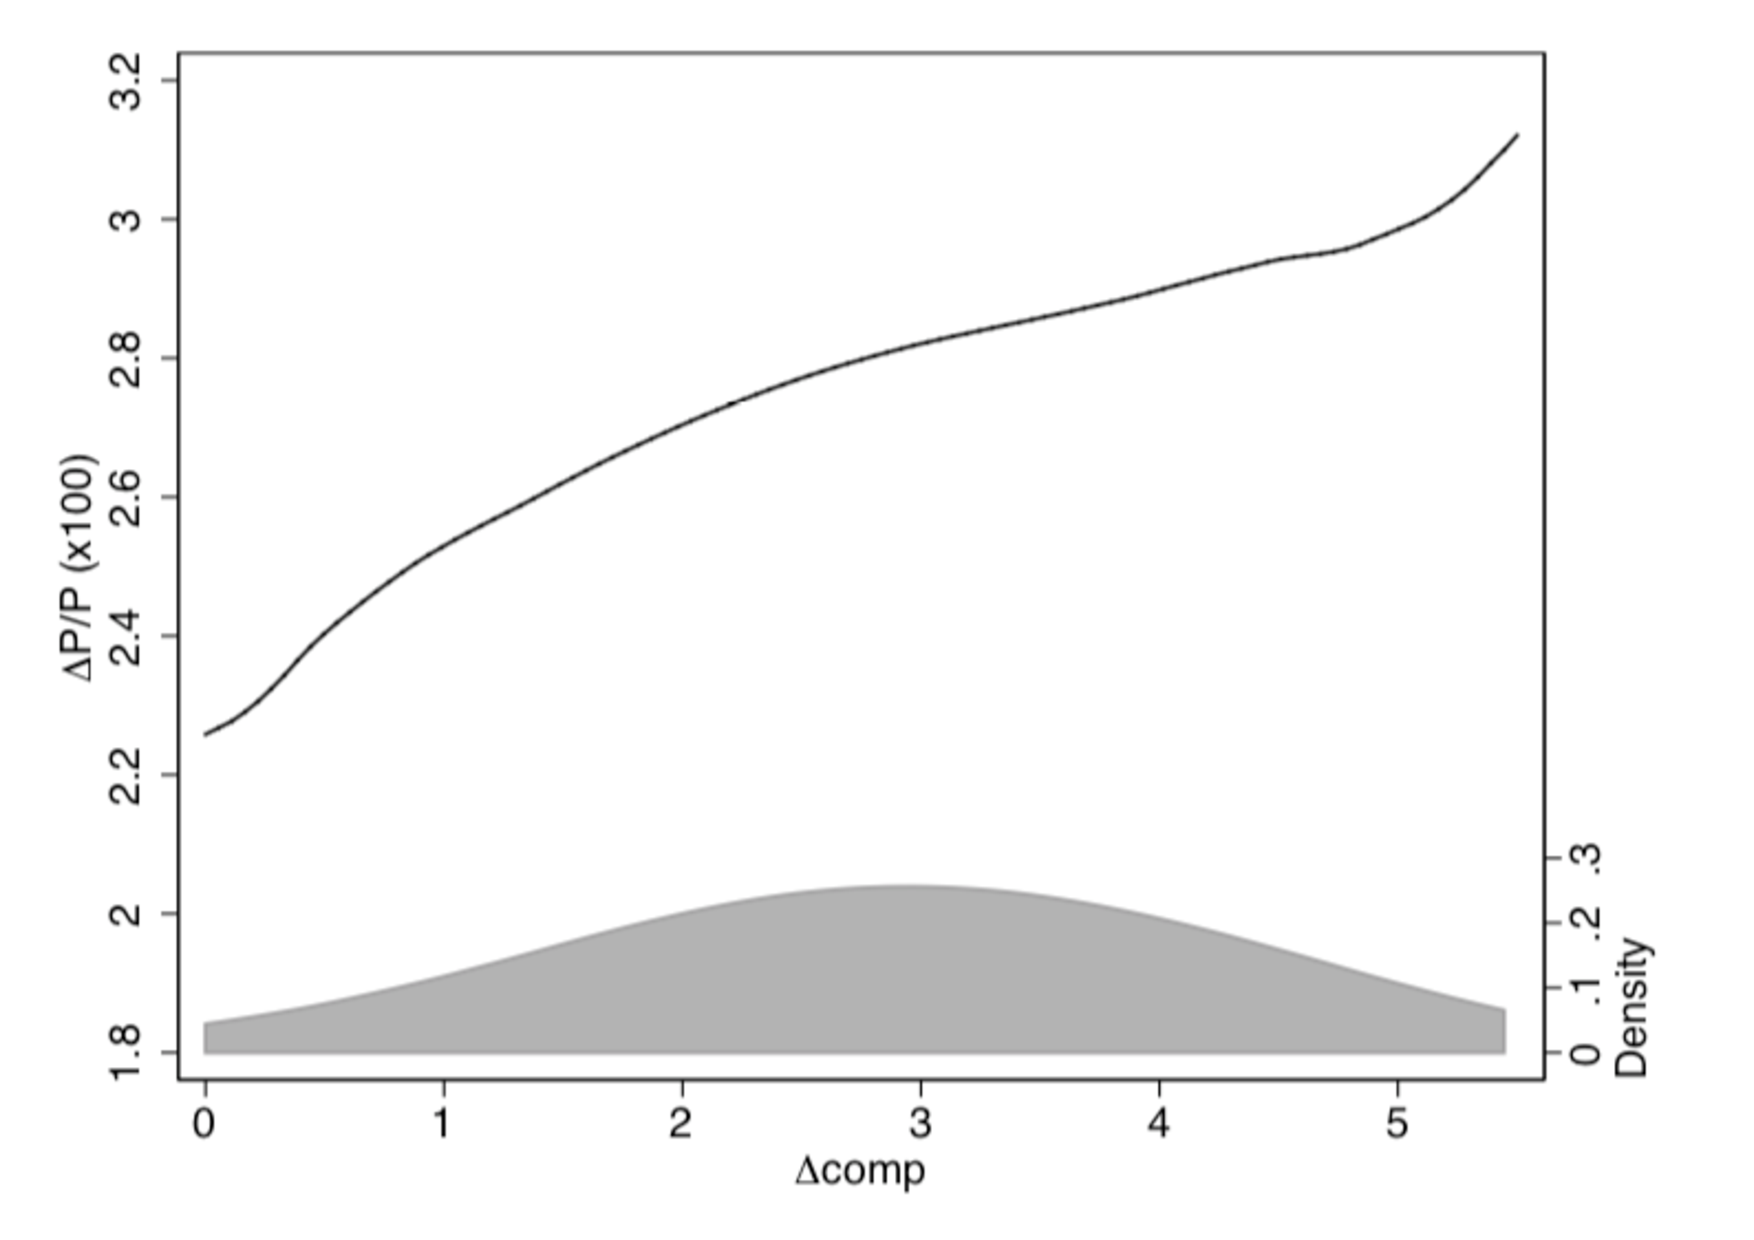
\includegraphics[width=0.85\textwidth]{cf1-a}
\caption{Change in Price vs. Change in Spatial Competition}
\end{figure}

}

\frame{\frametitle{Counterfactual \#1: changing farmers' outside option}
\begin{figure}[htbp]
\centering
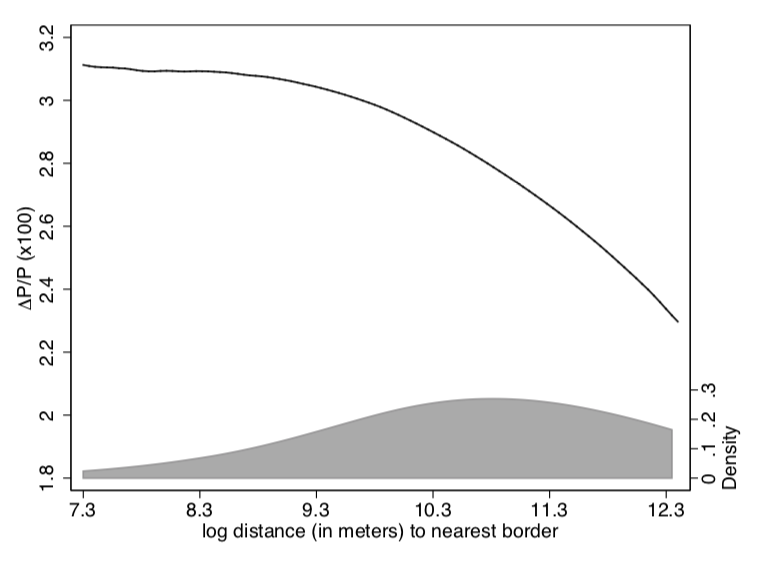
\includegraphics[width=0.85\textwidth]{cf1-b}
\caption{Change in Price vs. Distance to Nearest Border}
\end{figure}

}

\frame{\frametitle{Other counterfactuals}
\begin{table}
\centering
\caption{\textbf{Summary of Counterfactual Exercises}}
Change in farmer prices (\%)
\begin{tabular}{lrrrr}
\hline
& \multicolumn{2}{c}{Median} & \multicolumn{2}{c}{Mean} \\
& \textit{Fall }& \textit{Spring} &\textit{ Fall }& \textit{Spring}\\
\hline
\#1: Change outside option &1.75  & 2.50 & 2.74 & 2.65\\
\#2: \#1 + change market choice &8.35  & 5.82 & 12.60 & 10.72\\
\#3: \#2 + adjust retail prices & 5.98  & 6.21 & 9.62 & 9.56\\
\end{tabular}
\end{table}

}

\frame{\frametitle{Conclusion}
\begin{itemize}
\item Very cool paper: nice data work + simple, but powerful model!
\item Increasing spatial competition between intermediaries by removing interstate trade restrictions is good for farmers.
\end{itemize}

}


\section{Appendix}
\frame{
\vfill
\centering
\usebeamerfont{title}\textbf{Appendix}
\vfill
}

\frame{\frametitle{Causal estimates}
\begin{itemize}
\item Basic idea: choose market pairs that are close together but separated by a border 
\item Factors that affect price (other than spatial competition) should be similar for the market pairs. 
\item For each market pair $(m,m')$ estimate:
\begin{align*}
\Delta \log p^f_{cmdt} = \beta_1(\Delta \text{comp}_m) + \gamma_{ss'} + \tilde \e_{cmdt}
\end{align*}
\end{itemize}

}



\frame{\frametitle{Causal estimates}
\begin{table}
\centering
\caption{Border Discontinuity Regressions}
\begin{tabular}{lrrr}
\hline
& \multicolumn{3}{c}{Distance between market pairs (km)} \\
& $<25$ & $<30$ & $<35$ \\
\hline
$\hat{\beta}_1$ &0.025 & 0.035 & 0.036\\
Robust std. err. & 0.011 & 0.013 & 0.009\\
\end{tabular}
\end{table}
}

\frame{\frametitle{Estimation + calibration}
\begin{itemize}
\item Parameterize $\tau$:
\begin{align*}
&\tau_{mkct} = 
\begin{cases}
1 &\text{ if } m=k\\
1+ A\cdot d_{mk} + \e_{mct} & \text{ if } m \neq k\\
\infty & \text{ if } m, k \text{ in diff states}
\end{cases}\\
&\e_{mct} \sim \N(0,\sigma^2)
\end{align*}
\item Estimate $(\delta, \sigma^2, A)$ using SMM.
\end{itemize}

}

\frame{\frametitle{Model fit}
\begin{figure}[htbp]
\centering
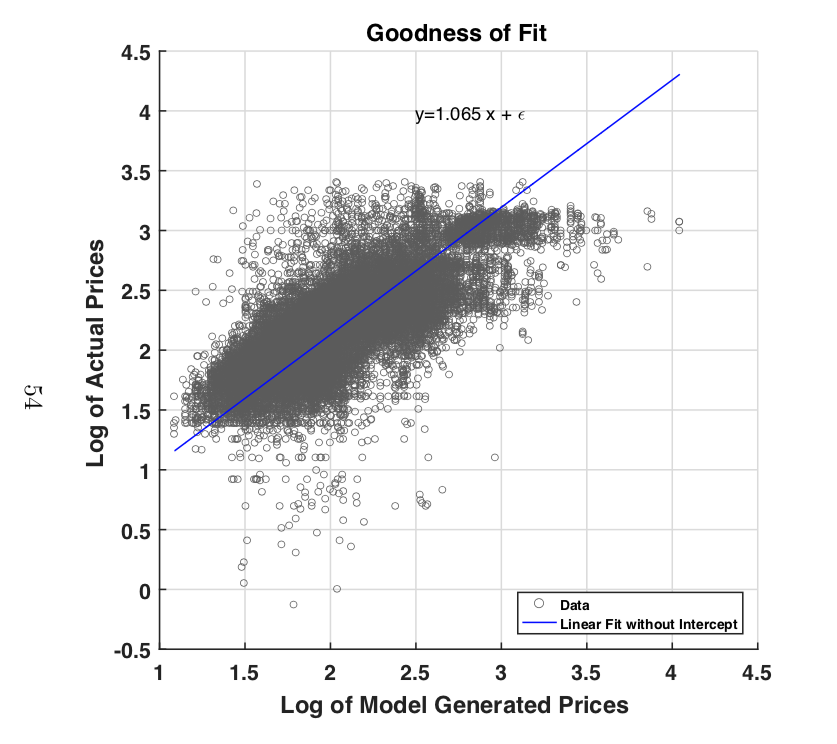
\includegraphics[width=0.8\textwidth]{fit}
\label{default}
\end{figure}

}

\frame{\frametitle{Counterfactual \# 2: Allow farmers to sell at different market}
\begin{figure}[htbp]
\centering
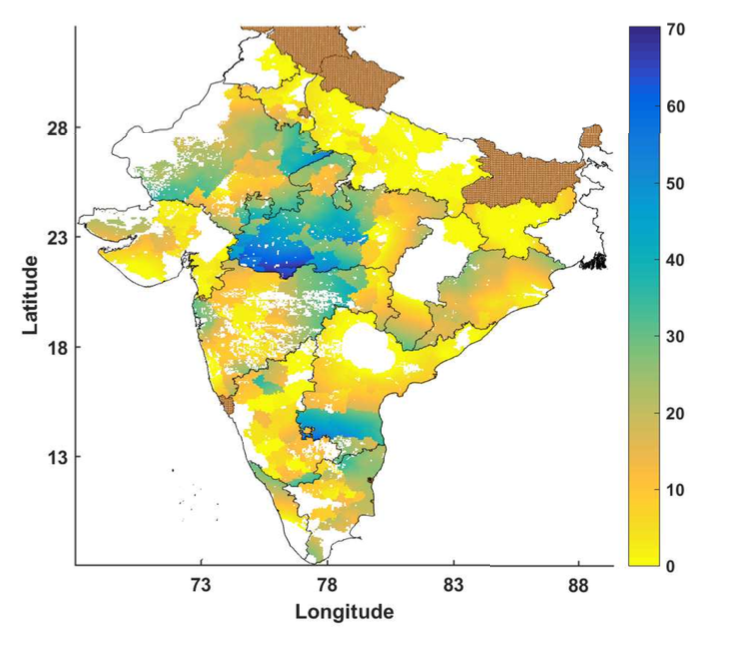
\includegraphics[width=0.7\textwidth]{cf2}
\label{default}
\end{figure}
}

\frame{\frametitle{Counterfactual \# 3: Allowing retail prices to adjust}
\begin{figure}[htbp]
\centering
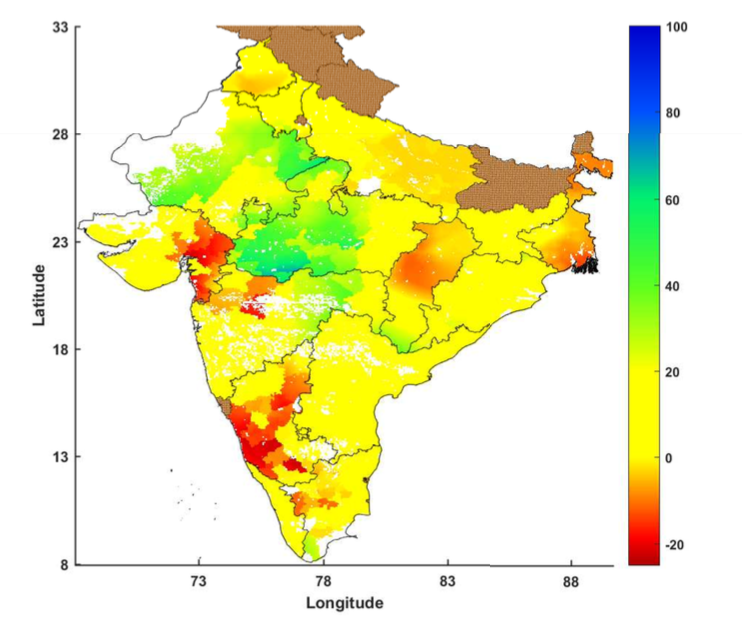
\includegraphics[width=0.7\textwidth]{cf4}
\label{default}
\end{figure}
}





\end{document}
